\documentclass[aspectratio=169]{beamer}
\usepackage[utf8]{inputenc} % codificacao de caracteres
\usepackage[T1]{fontenc}    % codificacao de fontes
\usepackage[english]{babel}  % idioma
\usepackage{graphics,amssymb,amsfonts,amsmath,xfrac}
\usepackage{tikz}
\usepackage{enumerate,hyperref}
\usepackage{palatino}	% Fonte sem serifa
\usepackage{ragged2e}	% Paragrafo justificado
%\usepackage{minted}	% Highlight para codigos de programacao
\usepackage{booktabs} % tabelas
\usepackage{multicol}
\usepackage{multirow}
%\usepackage[table]{xcolor}


% Veja mais temas e cores em http://www.hartwork.org/beamer-theme-matrix/
\usetheme{Montpellier}         % tema
\usecolortheme{orchid}      % cores
\usefonttheme[onlymath]{serif} % fonte modo matematico
% Colocando numero de paginas no slide
\setbeamertemplate{footline}[frame number]



\DeclareGraphicsExtensions{.pdf,.jpg,.png} % compilamos apenas com pdflatex
\graphicspath{{figuras/}} % caminho onde as figuras estarao disponiveis




% ---------------------------------------------------------------------------- %
% T�tulo                                                                       %
% ---------------------------------------------------------------------------- %

\title[\sc{Teoria de Circuitos Eletrônicos 1}]{\LARGE Aula 13 - Exercise Class 4}
\author[Prof. Marcelino Andrade]{Prof. Marcelino Andrade}
\institute{Faculdade UnB Gama} % opcional
\date{\today}

\begin{document}
\justifying % Paragrafo justificado
\pagebreak
\small
\begin{frame}
  \titlepage
\end{frame}


% ----------------- NOVO SLIDE --------------------------------
\begin{frame}{Contents\newline}

\tableofcontents
\begin{center}	
     		Introduction to Electric Circuits by James A. Svoboda, Richard C. Dorf, 9th Edition			
\end{center}	
\end{frame}

% ----------------- NOVA SECÇÂO -----------------------------
\section{CHAPTER 7 First-Order Circuits}
% ----------------- NOVO SLIDE --------------------------------
\begin{frame}[fragile]
	\frametitle{First-Order Circuit RL}
\begin{tabular}{ll}
	\begin{columns}
		\begin{column}{1\textwidth}  %%<--- here
		\textbf{Practice Problem 7.4} - For the circuit in Fig. below, find $i(t)$ for $t > 0$.\\
		\begin{center}
    			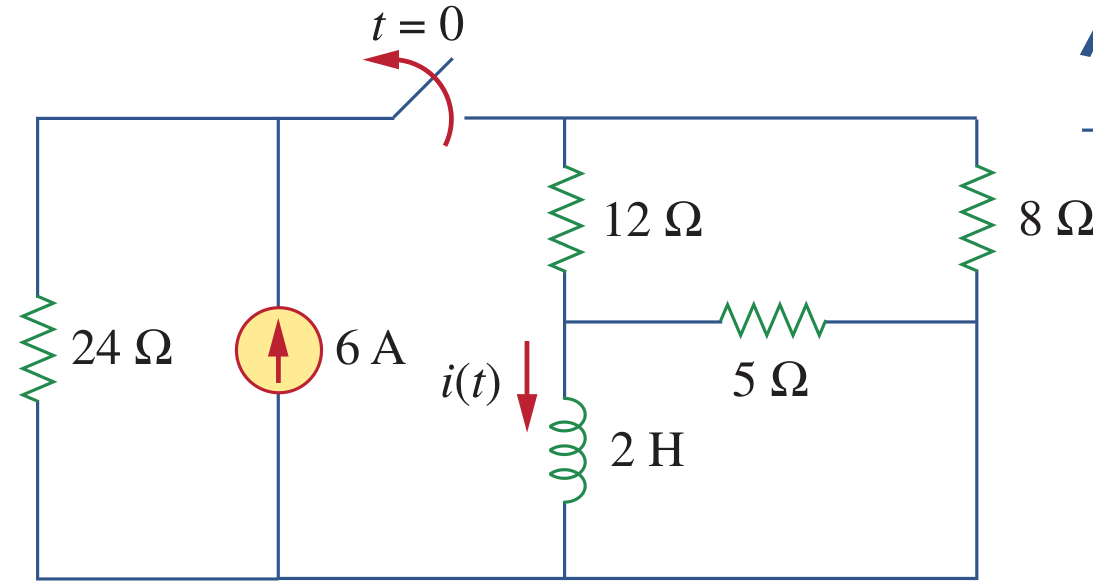
\includegraphics[height=3.6cm]{figure1.png}	
		\end{center}	
		\scalebox{0.8}{Answer: $2e^{-2t} \ A, \ t>0$.}
		\end{column}
	\end{columns}
\end{tabular}
\end{frame}

% ----------------- NOVO SLIDE --------------------------------
\begin{frame}[fragile]
	\frametitle{Step Response of an First-Order Circuit}
\begin{tabular}{ll}
	\begin{columns}
		\begin{column}{1\textwidth}  %%<--- here
		\textbf{Practice Problem 7.12} - The switch in Fig. below has been closed for a long time. It opens at
$t=0$. Find $i(t)$ for $t>0$.\\
		\begin{center}
    			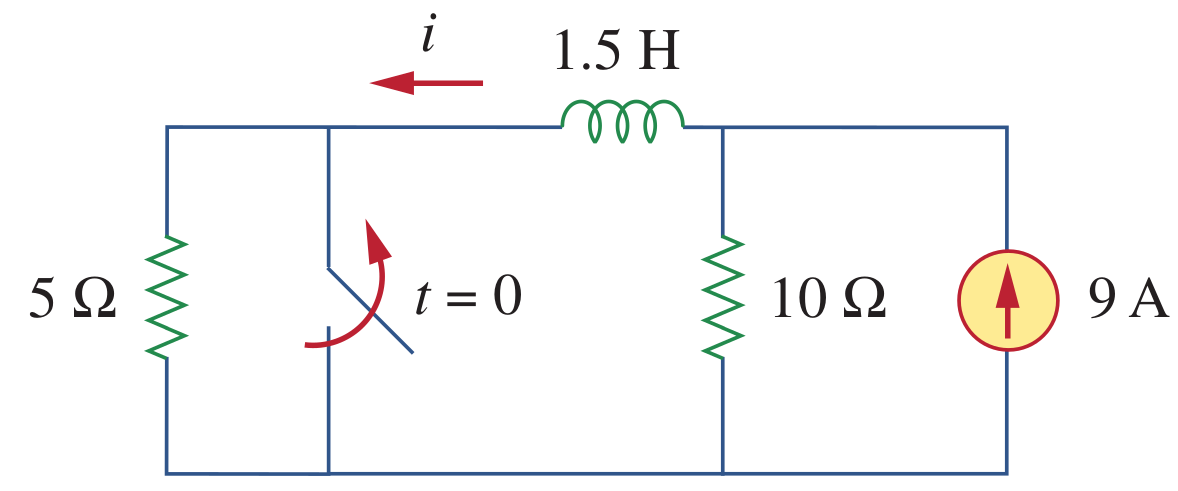
\includegraphics[height=3.6cm]{figure2.png}	
		\end{center}	
		\scalebox{0.8}{Answer: $i(t)=6+3e^{-10t} \ A \ for \ all \ t>0$.}
		\end{column}
	\end{columns}
\end{tabular}
\end{frame}

% ----------------- NOVA SECÇÂO -----------------------------
\section{CHAPTER 8 Second-Order Circuits}
% ----------------- NOVO SLIDE --------------------------------
\begin{frame}[fragile]
	\frametitle{Circuit Theorems}
\begin{tabular}{ll}
	\begin{columns}
		\begin{column}{1\textwidth}  %%<--- here
		\textbf{Example 8.9} - Find the complete response v and then $i$ for $t>0$ in the circuit of
Fig. below.\\
		\begin{center}
    			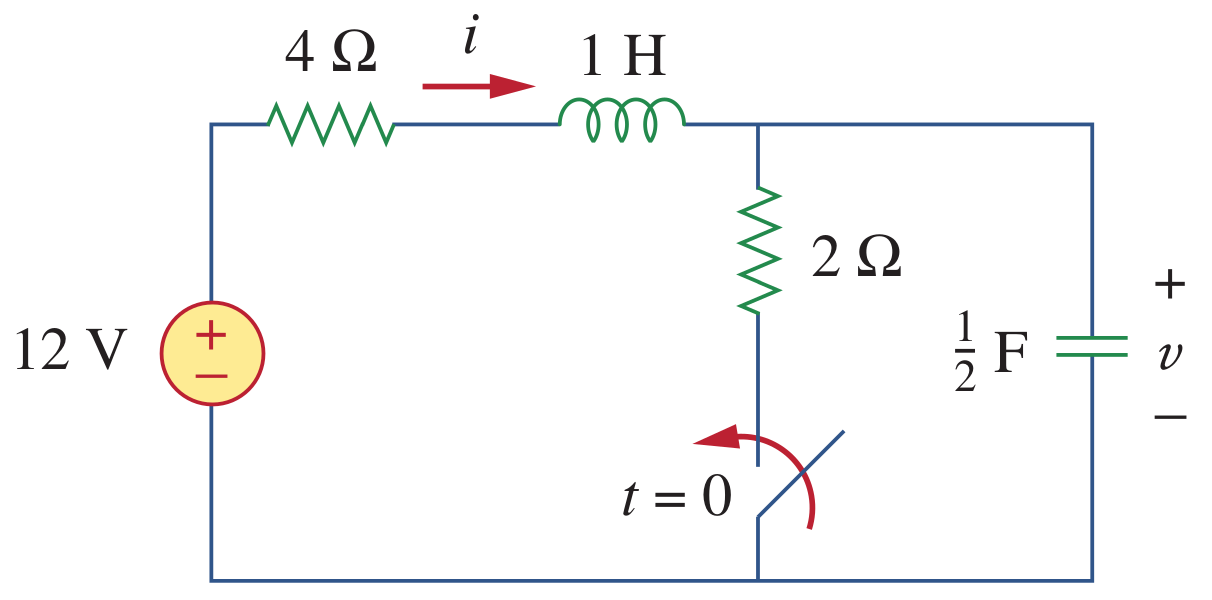
\includegraphics[height=3.6cm]{figure3.png}	
		\end{center}	
		\scalebox{0.8}{Answer: $v(t)=4+12e^{-2t}-4e^{-3t} \ V, \ t>0$}
		\end{column}
	\end{columns}
\end{tabular}
\end{frame}

% ----------------- NOVA SECÇÂO -----------------------------
\section{CHAPTER 16 Applications of the Laplace Transform}
% ----------------- NOVO SLIDE --------------------------------
\begin{frame}[fragile]
	\frametitle{Circuit Element Models}
\begin{tabular}{ll}
	\begin{columns}
		\begin{column}{1\textwidth}  %%<--- here
		\textbf{Example 16.4} - Consider the circuit in Fig. below. Find the value of the voltage
across the capacitor assuming that the value of $v_s(t)= 10u(t) \ V$ and
assume that at $t = 0$, -1 A flows through the inductor and +5 V is
across the capacitor.\\
		\begin{center}
    			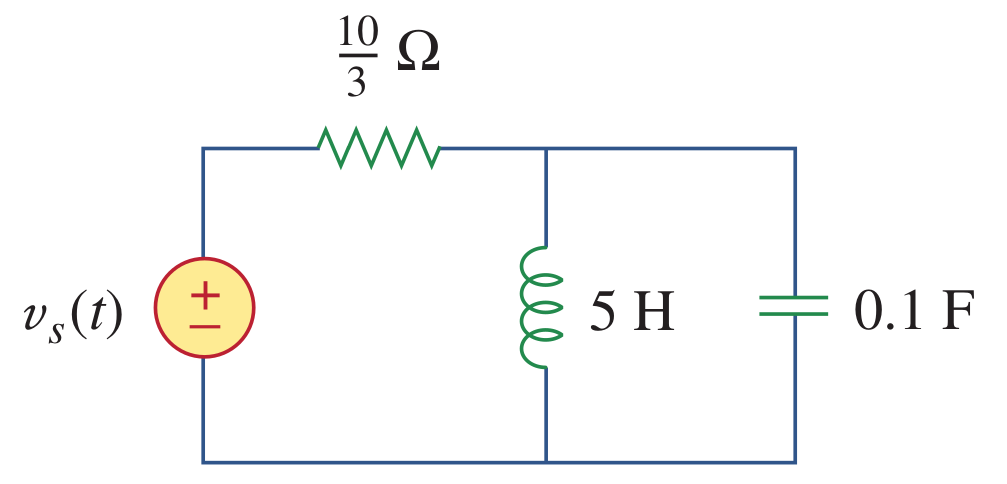
\includegraphics[height=3.6cm]{figure4.png}	
		\end{center}	
		\scalebox{0.8}{Answer: $v_c(t)=(35e^{-t}-30^{-2t})u(t)$}
		\end{column}
	\end{columns}
\end{tabular}
\end{frame}

% ----------------- NOVO SLIDE --------------------------------
\begin{frame}[fragile]
	\frametitle{Transfer Functions}
\begin{tabular}{ll}

\begin{columns}
  \begin{column}{1\textwidth}
\textbf{Problem 7.8-6} - Determine the transfer function $H(s) = \frac{I_1(s)}{I_o(s)}$ of the circuit in
Fig. below.\\
  \end{column}
\end{columns}\\

	\begin{columns}
		\begin{column}{1\textwidth}  %%<--- here
		\begin{center}
    			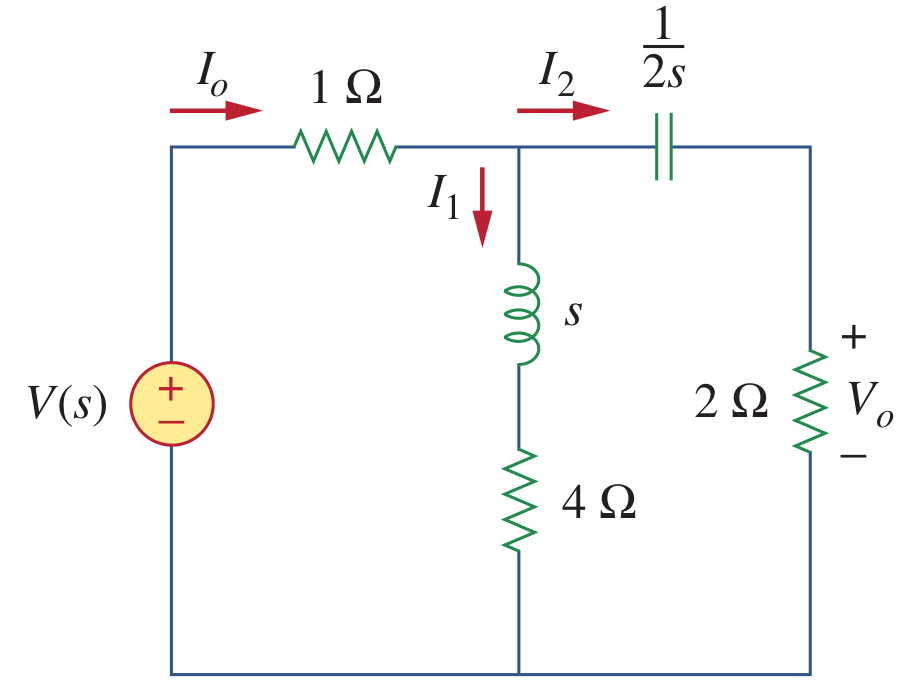
\includegraphics[height=3.6cm]{figure5.png}
		\end{center}	
\scalebox{0.8}{Answer: $H(s)=\dfrac{4s+1}{2s^2+12s+1}$}
		\end{column}

		
		
		
		
	\end{columns}
\end{tabular}
\end{frame}
% ----------------- NOVA SECÇÂO -----------------------------

\end{document} 






